\subsection{Crawler : S.R. Patra}
\subsubsection{Motivation}
The very first task was to collect data for our project. We decided to implement a focused crawler\cite{2ii35} for Rotten tomatoes website to collect information about different movies. Large collection of movies with credible reviews made Rotten Tomatoes a suitable candidate for us to get our data from. The goal was to start with a seed URL and extract all the yet unseen URLs on that HTML page along with the metadata about the movie such as movie name, director, producers,reviews etc. The process needs to be repeated for all the collected links.
\subsubsection{Approach}
For each page, the method \textit{CollectData} in the crawler read the HTML content line by line, only collecting the relevant information and disregarding all the other content that were not relevant to us. This was done with the help of an HTML parser which used \textit{Jsoup} library functions. Whenever relevant data were encountered, they were appended to an XML document. To find the movie URLs , Java's pattern matching functionality was being used which looks for a particular pattern of anchor texts which are specific to movie pages. The crawler architecture is shown in fig.\ref{fig:architecture}.

\begin{figure}[H]
    \centering
    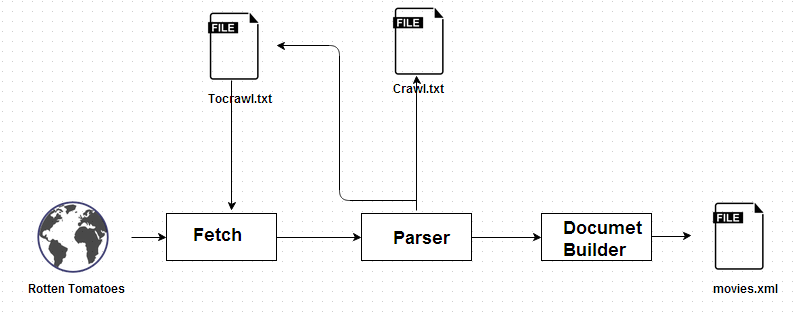
\includegraphics[width=4.0in]{crawler_arch.png}
    \caption{Crawler Architecture}
    \label{fig:architecture}
\end{figure}

\subsubsection{Challenges}
The main challenge was to encounter the non uniformity of the content in Rotten Tomatoes web pages. Some of the web pages contained all the information about the movies while in others, a few of the information fields were missing. The crawler was designed to scrap the HTML data in a way such that maximum amount of information can be retrieved. Another challenge was to make sure that the crawler is not blocked by the site. This was handled by building the crawler in a flexible way so that, during an iteration, the crawler will only crawl through a specific number of pages specified to it as a parameter. After each iteration, the URLs which are already crawlled and the URLs those are yet to be crawlled are written back to \textit{Crawl.txt} and \textit{Tocrawl.txt} respectively which will be used in the next iterations. Fig.\ref{fig:xmlFile} shows an entry in the \textit{movies.xml} file.

\begin{figure}[H]
    \centering
    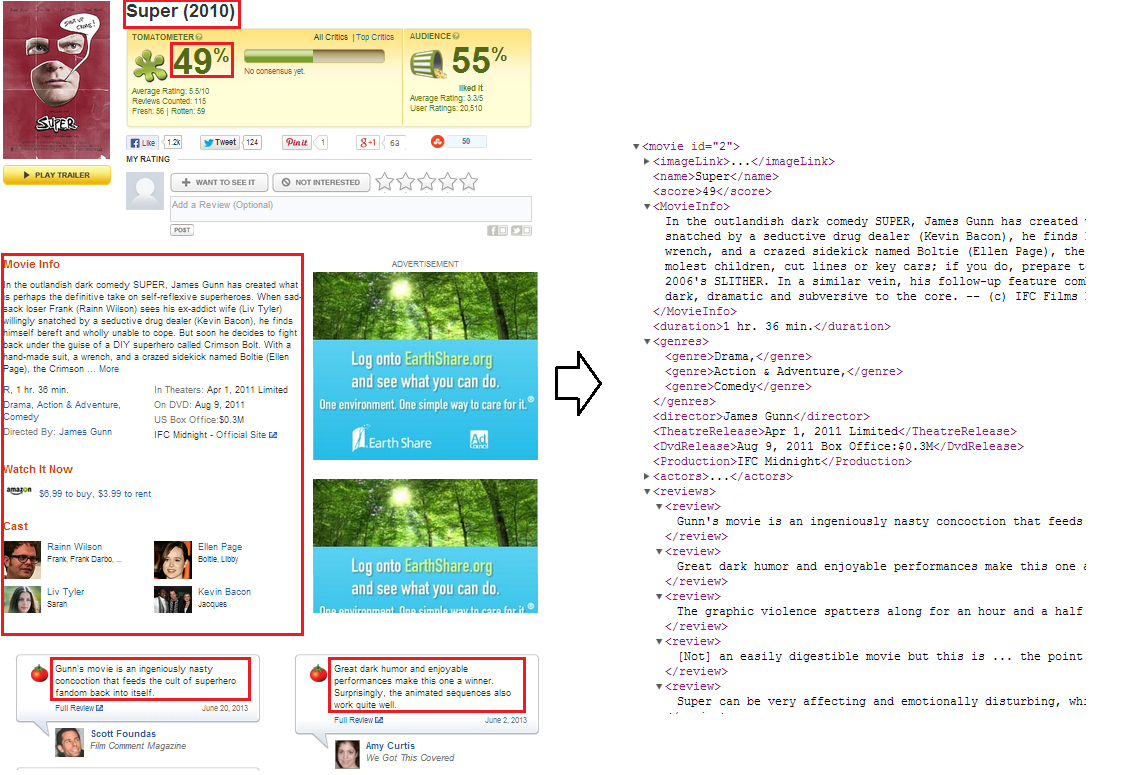
\includegraphics[width=4.5in]{rot.png}
    \caption{Collecting data from Rotten Tomatoes}
    \label{fig:xmlFile}
\end{figure}

\subsubsection{Evaluation \& Summary}
After several iterations, we collected 6227 movies each containing movie metadata and the reviews. We collected only top critics reviews because we feel that those are the most representative of all the reviews. As focused crawler parse all the content in documents and filter only the relevant content for the application, crawling took more time than a normal crawler would take. But the flexibility in the design of the crawler allowed us to run it in iterations so we did not face any issue regarding the time for crawling. We took 20 random samples from the file and compared the contents with the content in the site. In all the cases, we were able to capture all the relevant data needed for the search and sentiment analysis functionality.

\subsection{Lucene Search, Wildcard Queries \& Autocomplete : S.R. Patra}
\subsubsection{Motivation}
Lucene provides very rich library functions to implement indexing and search. So we implemented lucene search as a metric to evaluate our boolean and vector space model performances. 
\subsubsection{Approach}
Lucene.net library\cite{lucene} was used for generating the index and for getting the search results from the processed query. We limited our search results to be 10 top relevant results. Index was created for different fields to allow the user to search based on any criteria they want i.e. based on actor, director, genres etc. We also implemented the \textit{Autocomplete} feature to help the user with the query. This feature was developed in \textit{JQuery}\cite{jquery} and was implemented as a web service which queries the database about possible movie names after each input letter in the text box. 

\paragraph{}
Wild card queries\cite{wildcard} were used to provide query suggestions to the user when the user only knows parts of the terms in the query. The speech to text query assistance feature was also included using the HTML5 Webkit speech. All the features discussed above are shown in fig.\ref{fig:search}.
\begin{figure}[H]
    \centering
    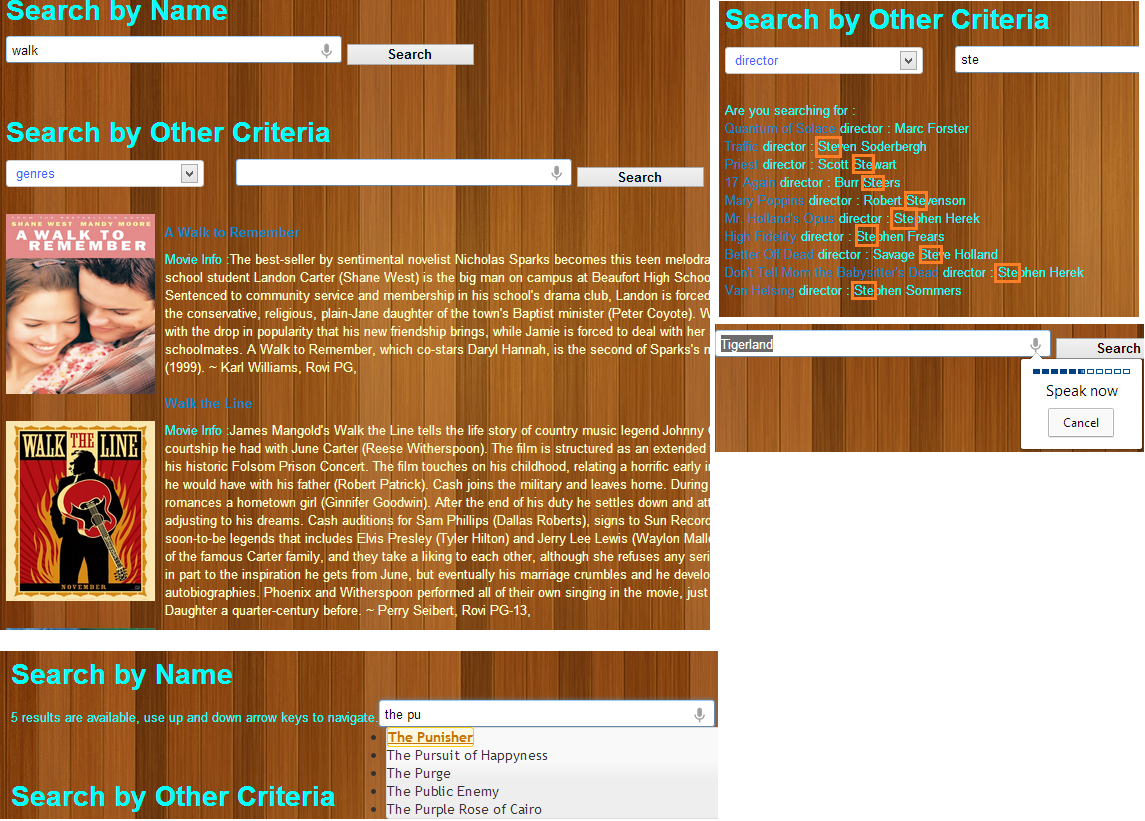
\includegraphics[width=4.5in]{search.png}
    \caption{Searching functionalities}
    \label{fig:search}
\end{figure}

\subsubsection{Evaluation \& Summary}
After trying a number of sample queries for different search criterias, we feel that the search provided quite relevant results in all the cases. The wildcard queries were also accurate in their suggestions and the users were able to retrieve relevant movie names based on parts of the search query terms. 